\documentclass[times, 10pt,twocolumn]{article}
%\usepackage{ucs}
\usepackage{amsmath}
\usepackage{amsfonts}
\usepackage{amssymb}
%\usepackage{glossary}
%\usepackage{ucs}
\usepackage{listings}
%\usepackage{fontenc}
\usepackage{graphicx}
\usepackage{float}
\usepackage{color}
%\usepackage{tipa}
\usepackage{url}
\usepackage{hyperref}
%\usepackage{wrapfig}
%\usepackage{subfig}
\usepackage[left=1cm, top=1cm, right=1cm, left=1cm, nohead, nofoot]{geometry}
\title {RMI-based chat application: Papinho}
\author{Andon Tchechmedjiev, Jander Nascimento}

\begin{document}
\maketitle
\section{Presentation}
\section{Remote interfaces}

\paragraph{}
We will first define the remote interfaces we used, as they constitute the basis of our application. There is one remote interface for the server application and one for the client application.
\paragraph{}
The architecture we have chosen for our application is a classical server centric one. Namely, all the clients are synchronized to a central state kept on the server. All messages be they public or private messages, will always transit through the server, where logging will occur.

\subsection{Chat server side}
\paragraph{}

The server provides the services in the table \ref{tab:serverprovide}. Those services are provided in order to allow the client to comunicate between other clients and the server itself. 

  \begin{table}[H]
  \begin{center}
      \begin{tabular}{ | l | p{5cm} |}
      \hline
      Method & Summary \\ \hline
      addClient & Add a client to the list of clients in the server side \\ \hline 
      removeClient & remove a client from the list of clients \\ \hline
      sendMessage &  broadcast certain message to all the clients, or for a specific client\\ \hline
      clientNameChange & Change the user's login \\ \hline
      \end{tabular}
  \end{center}
  \caption{Server Side: Provided methods}
  \label{tab:serverprovide}
  \end{table}

\subsection{Chat client side}

The client must provide some methods so the server can inform the client about new messages, user renaming, etc.  
  \begin{table}[H]
  \begin{center}
      \begin{tabular}{ | l | p{5cm} |}
      \hline
      Method & Summary \\ \hline
      addClient & Add a client to the list of clients in the client side \\ \hline 
      removeClient & remove a client from the list of clients in the client side \\ \hline
      receiveMessage & Add a new message to the main window \\ \hline
      receivePrivateMessage &  Add a new message to a private chat window \\ \hline
      changeClientName & Change the username in the list of clients on the client side \\ \hline
      \end{tabular}
  \end{center}
  \caption{Client Side: Provided methods}
  \label{tab:clientprovide}
  \end{table}

\section{History and persistence}

In order to manage the persistence, the main design pattern used was a creational pattern {\it Proxy}. The main goal of this pattern is to decide which instance to generate.
On the current implementation the persistence method used was the {\it serialization of the object to disk}, what is also called as {\it bean serialization}. 

\section{Graphical User Interface}

The Graphical User Interface(GUI) allow the user to interact with the application in a more intuitive way. 
The GUI was implemented using Java Swing libraries. An example of the interface can be seem in the Figure \ref{fig:papinho1}

\begin{figure} [H]
    \centering
%    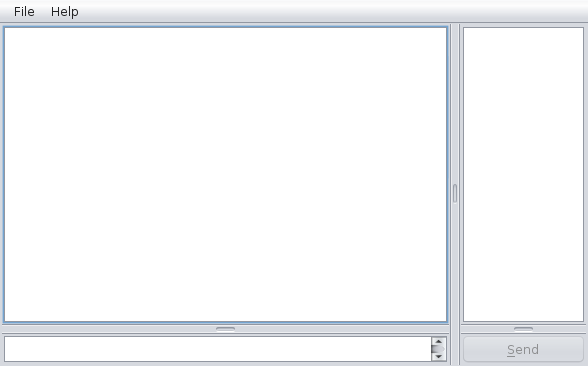
\includegraphics[scale=0.3]{img/mainscreen}
    \caption{Main Window} 
    \label{fig:papinho1}
\end{figure}

\section{Networking and security issues}

Since Java Virtual Machine runs inside a sandbox, term coined by sun. The application must explicity tell the JVM which kind of connections are allows and which hosts are allowed to do so.
To specify this information is necessary to write a policy file. In this file we specify the permission, host, port and actions. 

In the example \ref{policyfile} the policy allows socket connections from any host to any port. 


\begin{lstlisting}[caption={Policy file},label=policyfile]
grant {
  permission java.net.SocketPermission "*:*", "accept,listen,connect,resolve";
};
\end{lstlisting}


\end{document}
